\newpage
\chapter{Design Changes}
\label{chap:design_changes}
% what major design changes have been introduced since the CDR report? Argument why these changes were necessary. Also, will be good to include test results (functionality, weight, performance etc.) which are not documented in the CDR report.


\section{Project Schedule, Resources and Goals}
%responsible: Morten

Project initially substantially delayed due to bureaucratic challenges in course registration and release of project budget.

Reduction in project team resources due to people leaving for 3rd semester in June 2012. 

Reformulation of project goals due to reduction of people and initial project delays.

New project manager 

New team member (Omair) working on new subsystem (COM).

Budget for each of four remaining students increased from 2000 SEK to 2500 SEK.


\section{Electrical Power Subsystem}
%responsible: Morten

MPPT not implemented due to time limitation.

SAR not implemented due to time limitation.

Solar cells not ordered due to budget limitations and lack of time to integrate these in design.

Battery failure due to heavy discharge - people must be aware of limitations on Li-ion batteries and any electronics connected to battery must prevent this situation.

Updated mass specifications on units.

Challenges in thermal design to achieve specifications on battery. A passive design has been made. Specify test results. Suggestion to add a heater or have a winter + summer configuration of the insulation.

Inclusion of 3.3V regulated output - mainly due to limitations on BeagleBoard which is not compatible with 5V?

Battery Charge Regulator:
Chosen battery may supply 66A continuously or 88A. Main limitation of EPS power output is due to ratings on power diode (20A), power connectors (19A) and wire (19A, 11.5A using ECSS derating). Also, PCB trace thickness may become impractically thick at higher current ratings. To improve power rating: use high power connectors, use thicker wire or several in parallel, use high power diode or two diodes in parallel. Use thicker PCB copper tracing, reduce trace length, increase trace width and improve thermal layout (lots of heat sinks).

\subsection{Battery Charge Regulator}

Additional telemetry data outputs added for BCR.

BCR on dedicated PCB and SAR + logic voltages regulator on separate PCB. 

BCR functionality fully verified along with all safety functions (UVLO, temperature monitoring + charge cut-off, charge regulation, short-circuit protection).

\begin{figure}[H]
\begin{minipage}[t]{\linewidth}
\centering
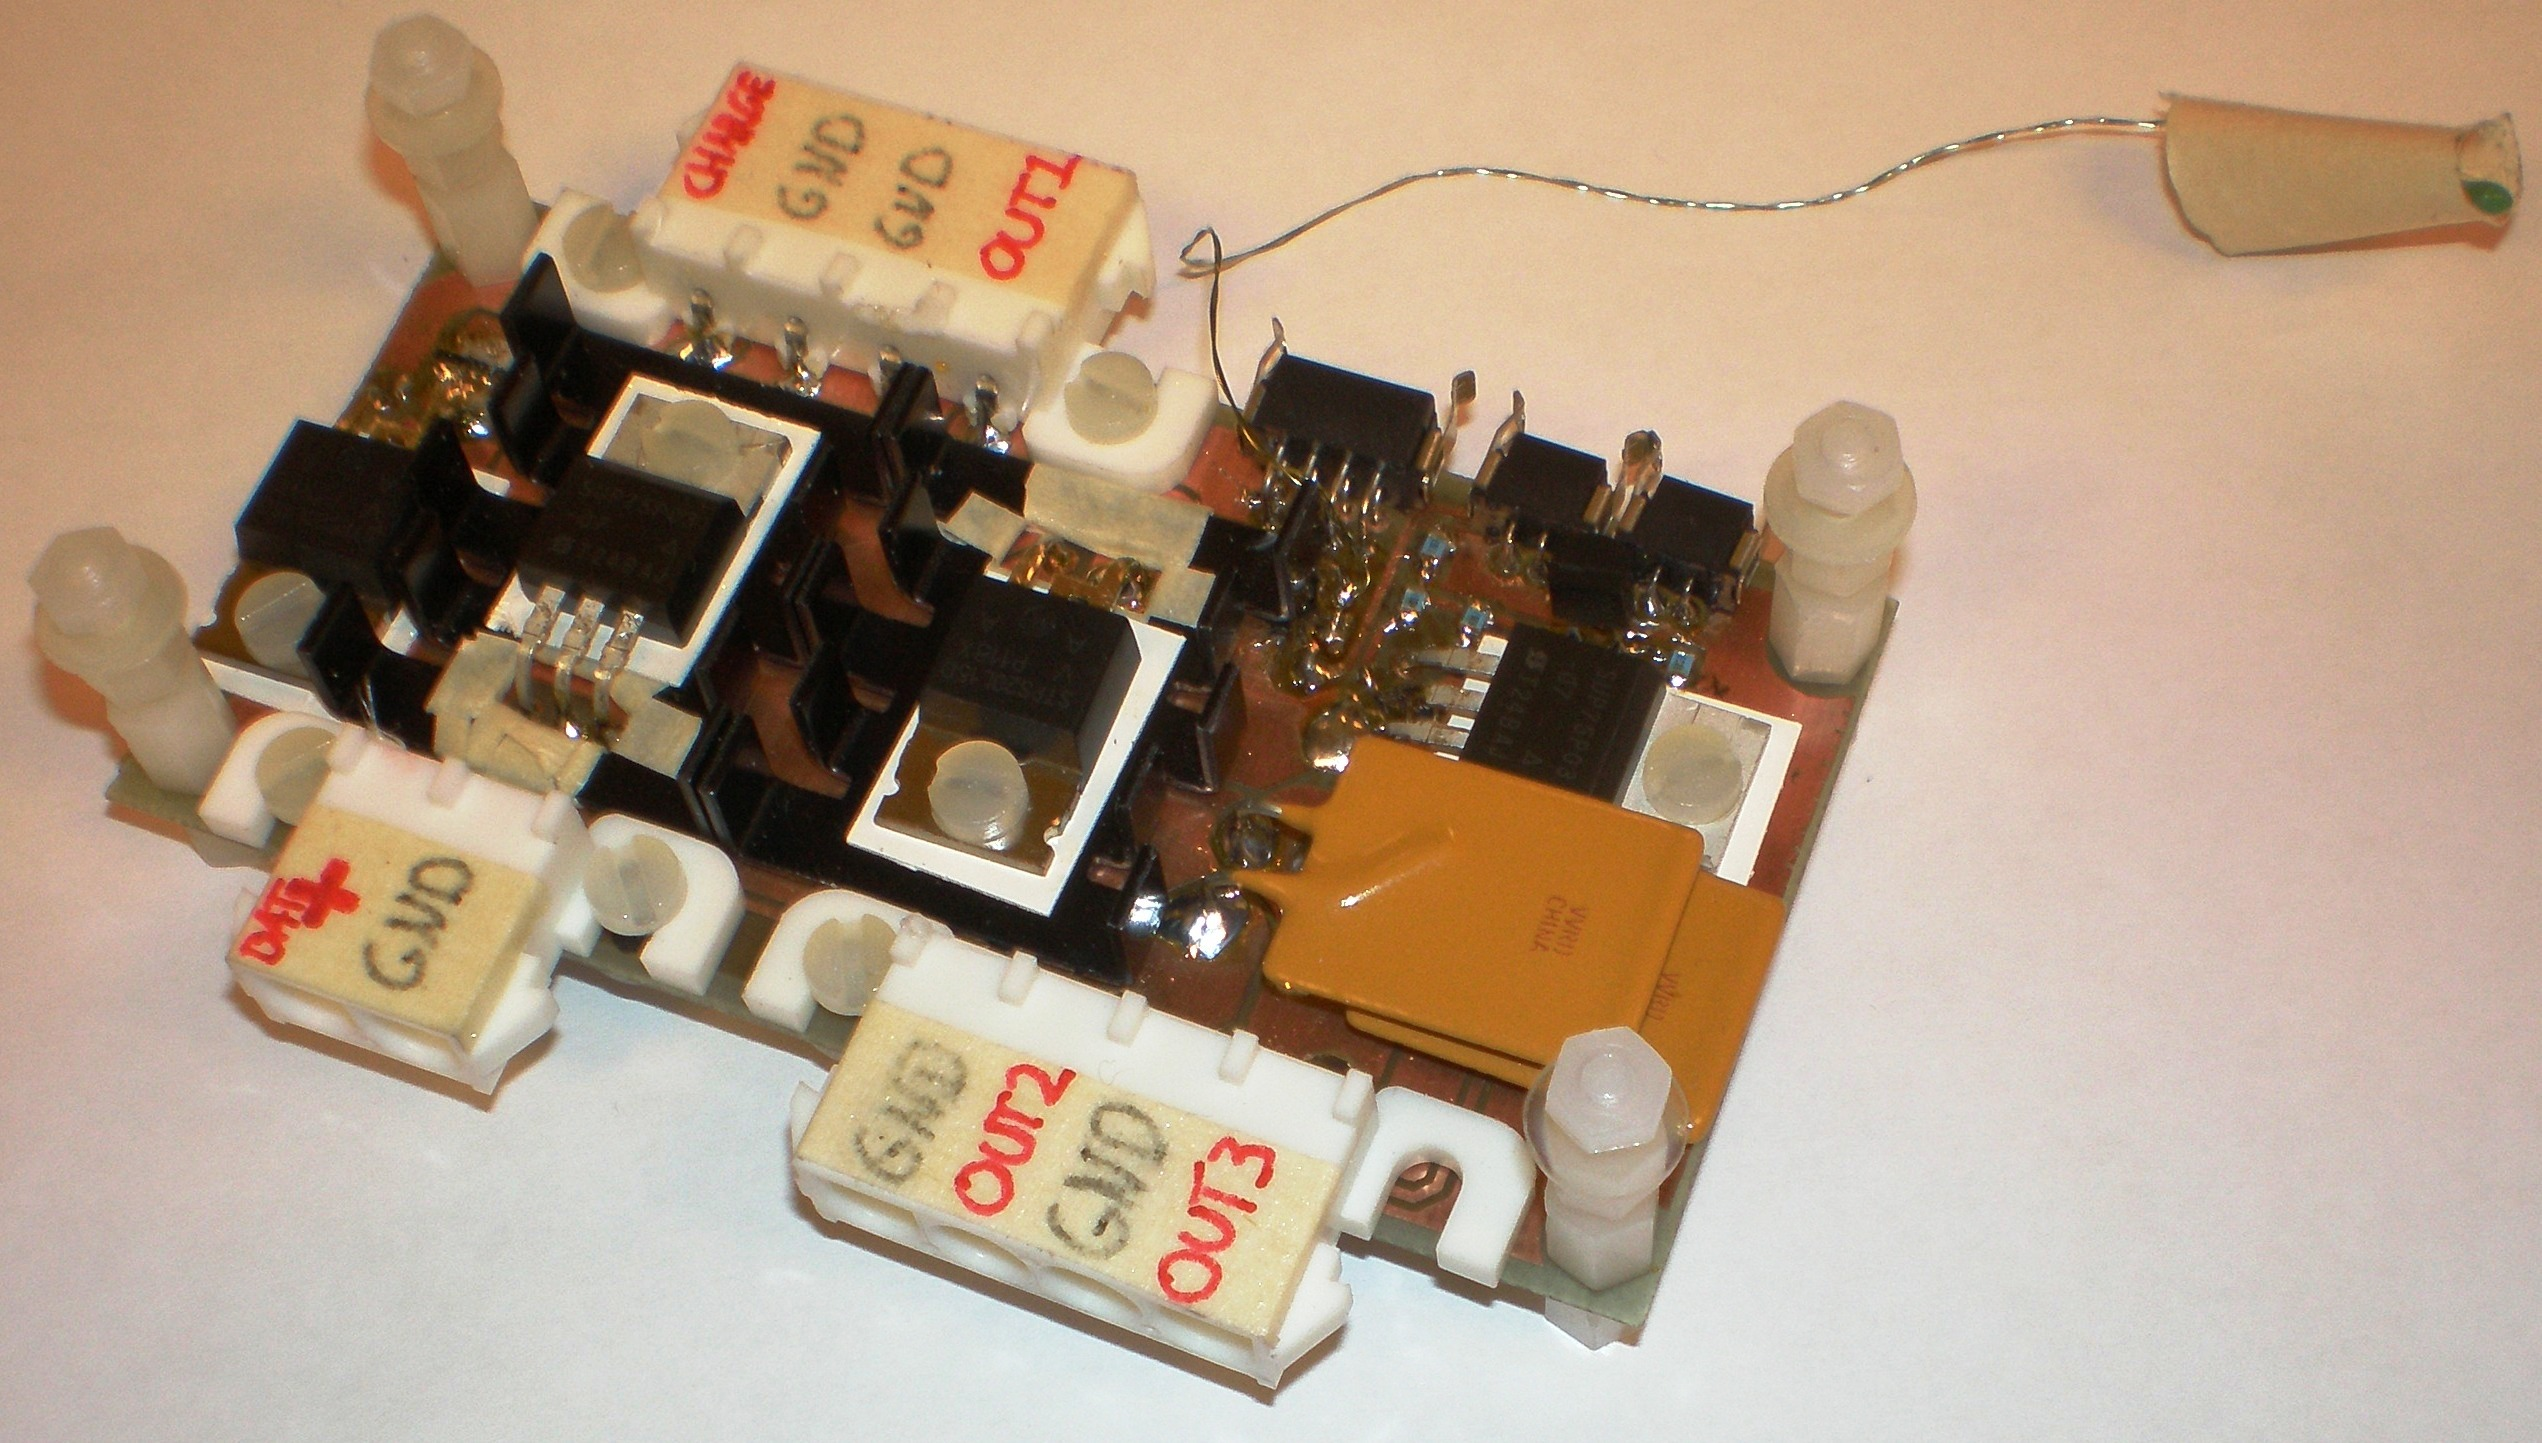
\includegraphics[width=0.7\textwidth]{figures/fig_BCR_top}
\end{minipage}
\vspace{2mm}
\begin{minipage}[t]{\linewidth}
\centering
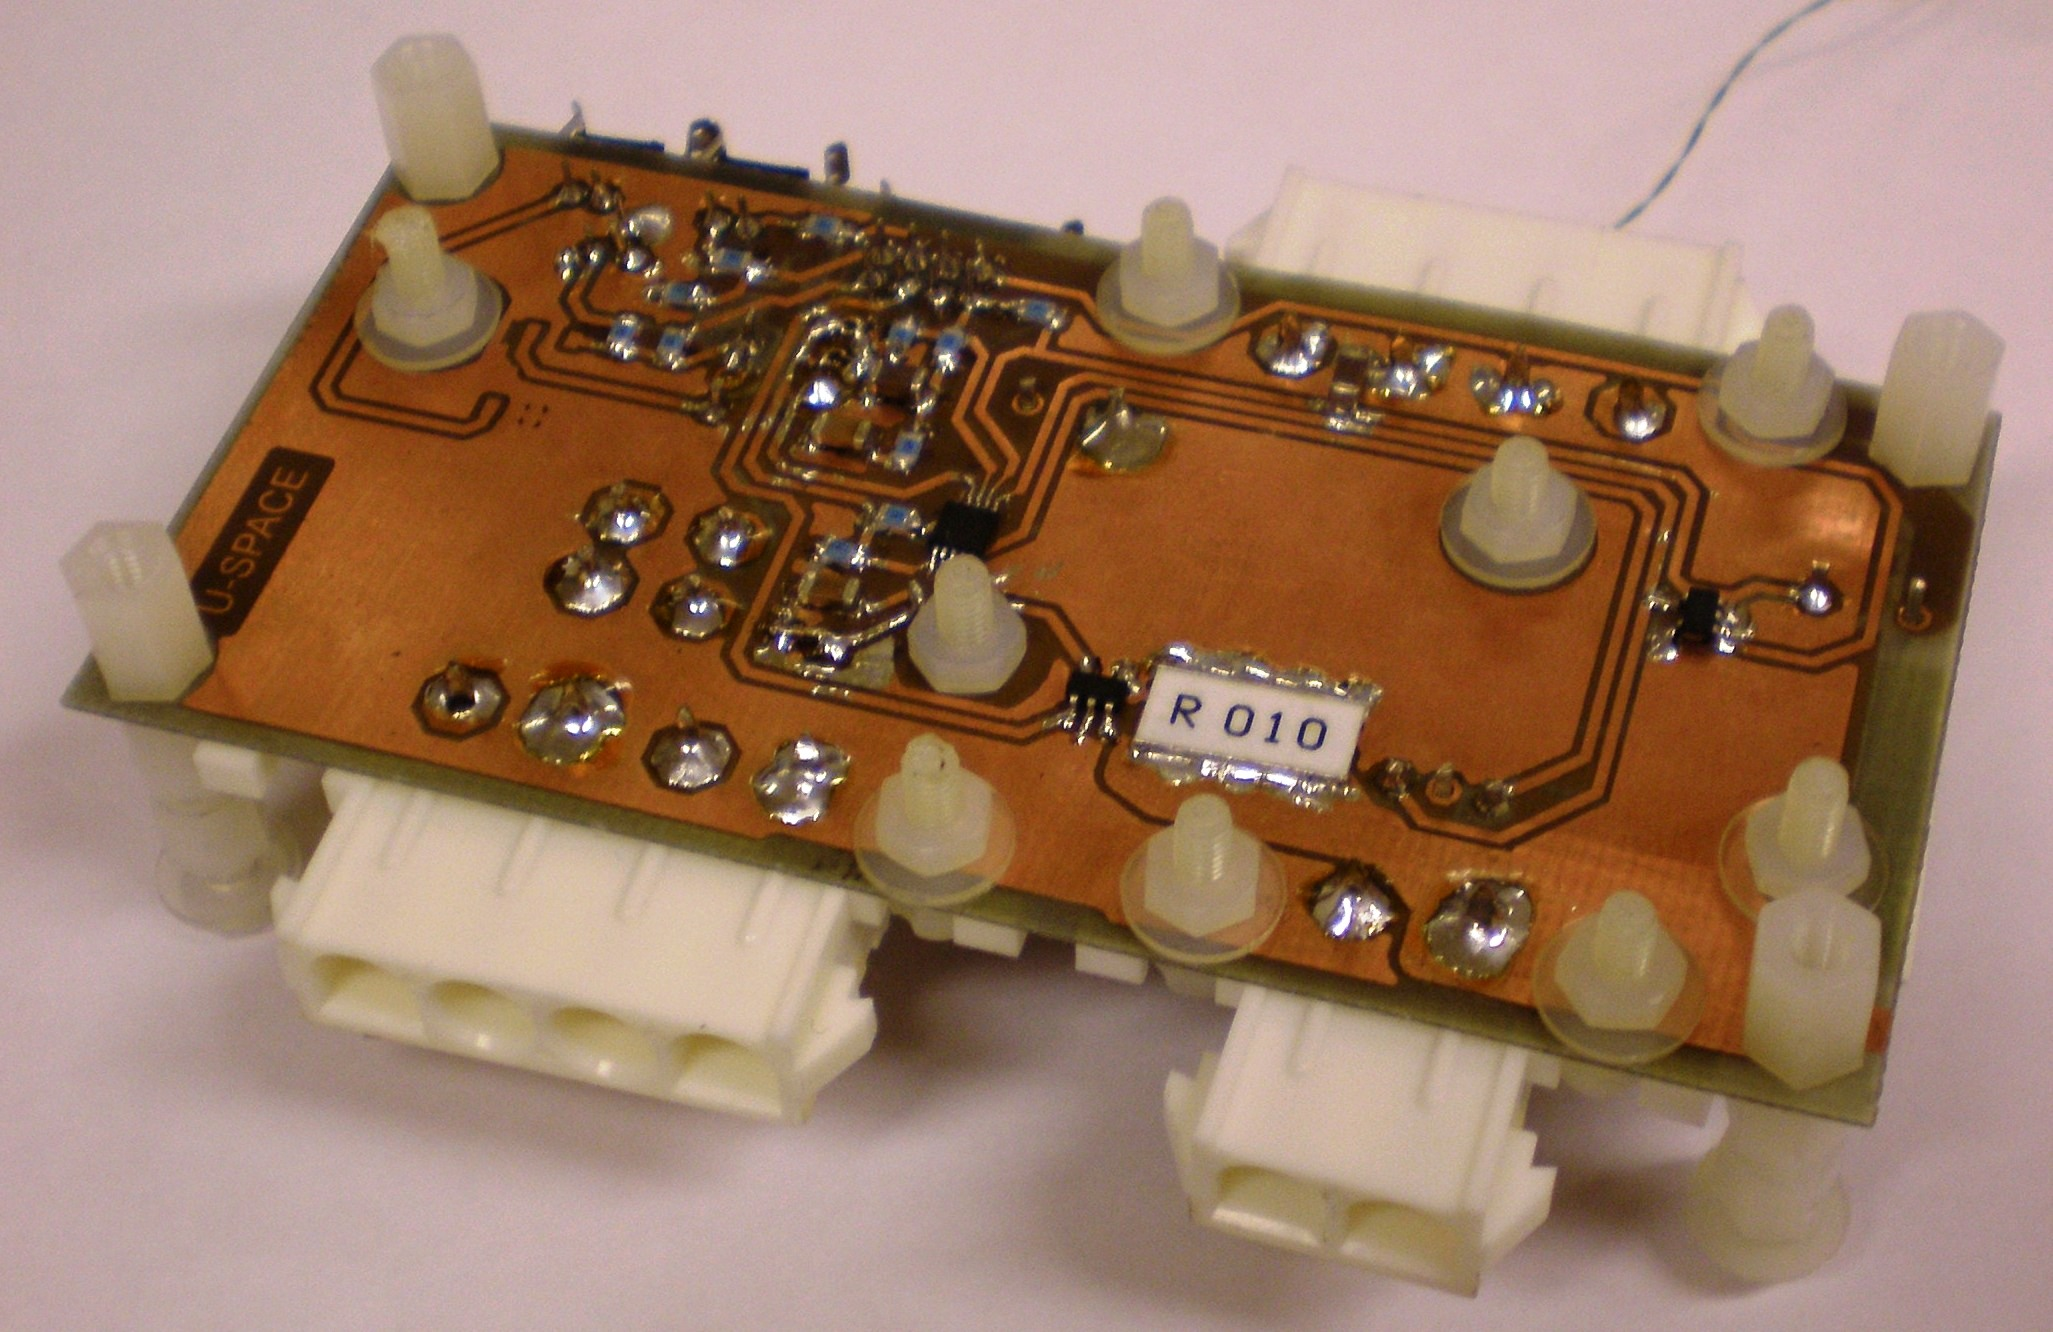
\includegraphics[width=0.7\textwidth]{figures/fig_BCR_bottom}
\end{minipage}
\caption{Battery Charge Regulator}
\label{fig:BCR_top_bottom}
\end{figure}

\begin{figure}[H]
\centering
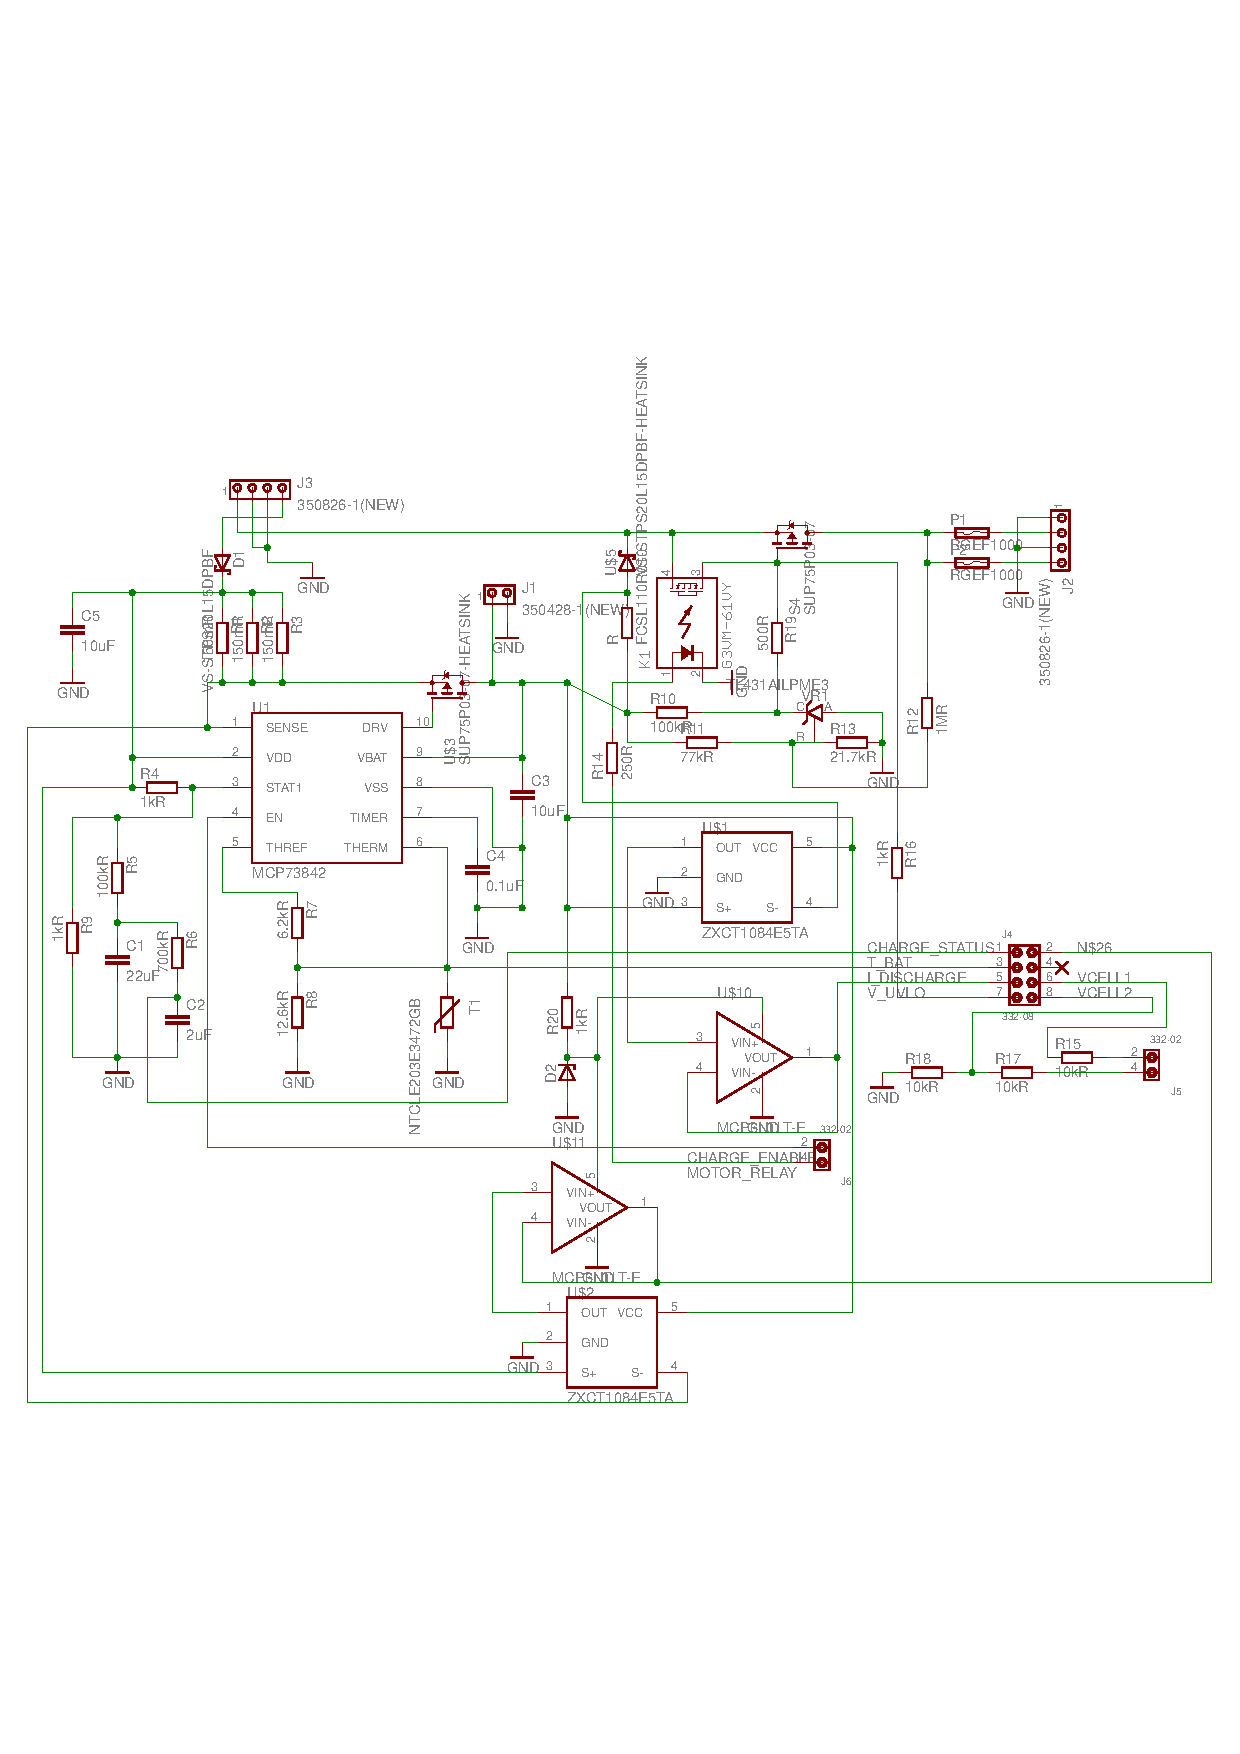
\includegraphics[width=\textwidth]{figures/fig_Schematic_BCR}
\caption{Schematic of the \acl{BCR}}
\label{fig:BCR_Schematic}
\end{figure}

\subsection{Solar Array Regulator}

Additional telemetry data outputs added for SAR.

\begin{figure}[H]
\begin{minipage}[t]{\linewidth}
\centering
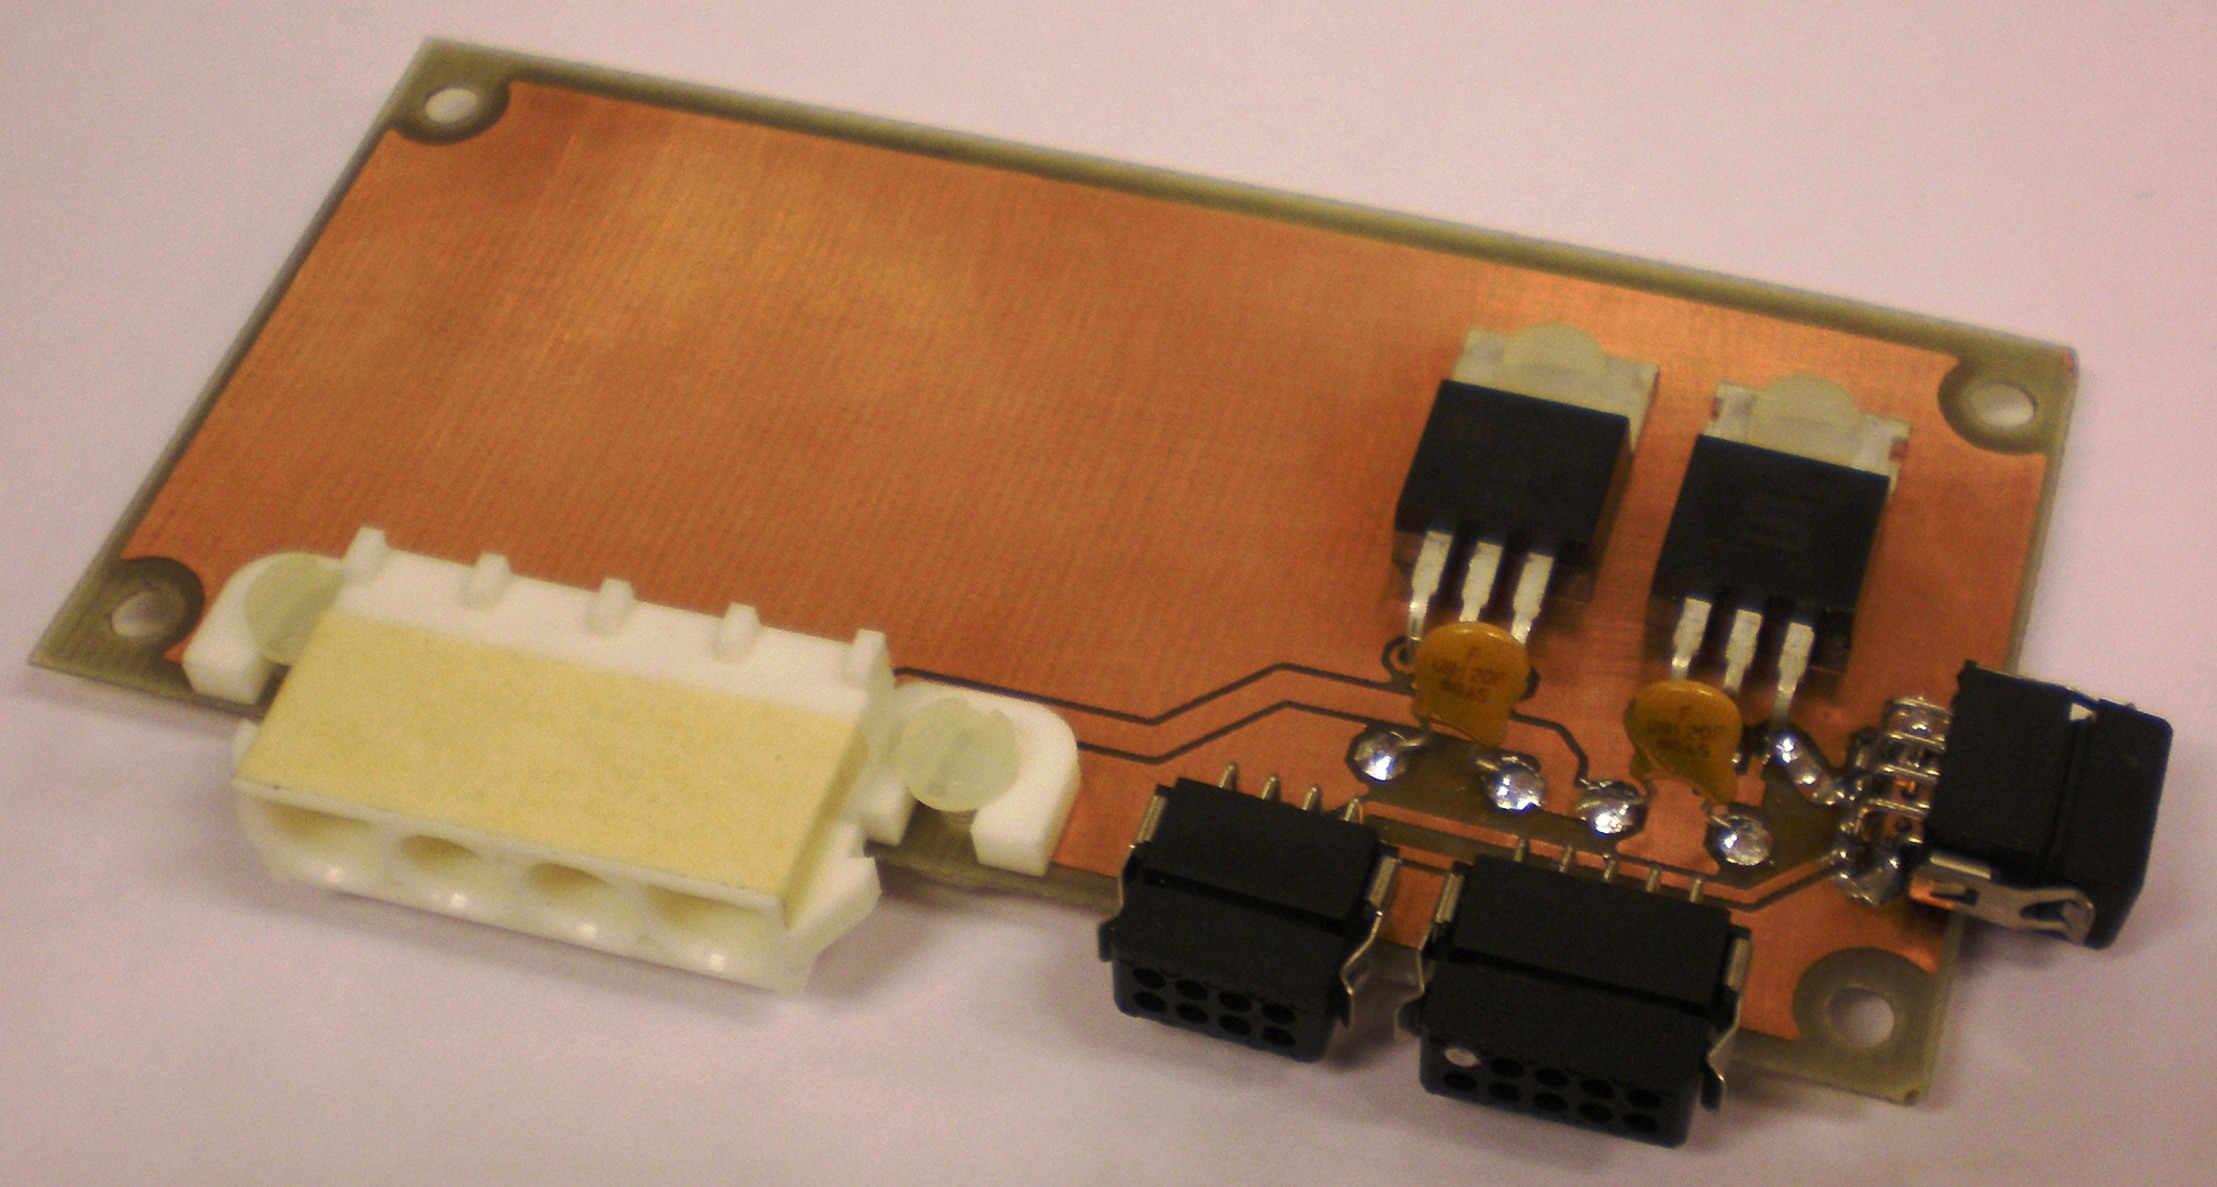
\includegraphics[width=0.7\textwidth]{figures/fig_SAR_top}
\end{minipage}
\vspace{2mm}
\begin{minipage}[t]{\linewidth}
\centering
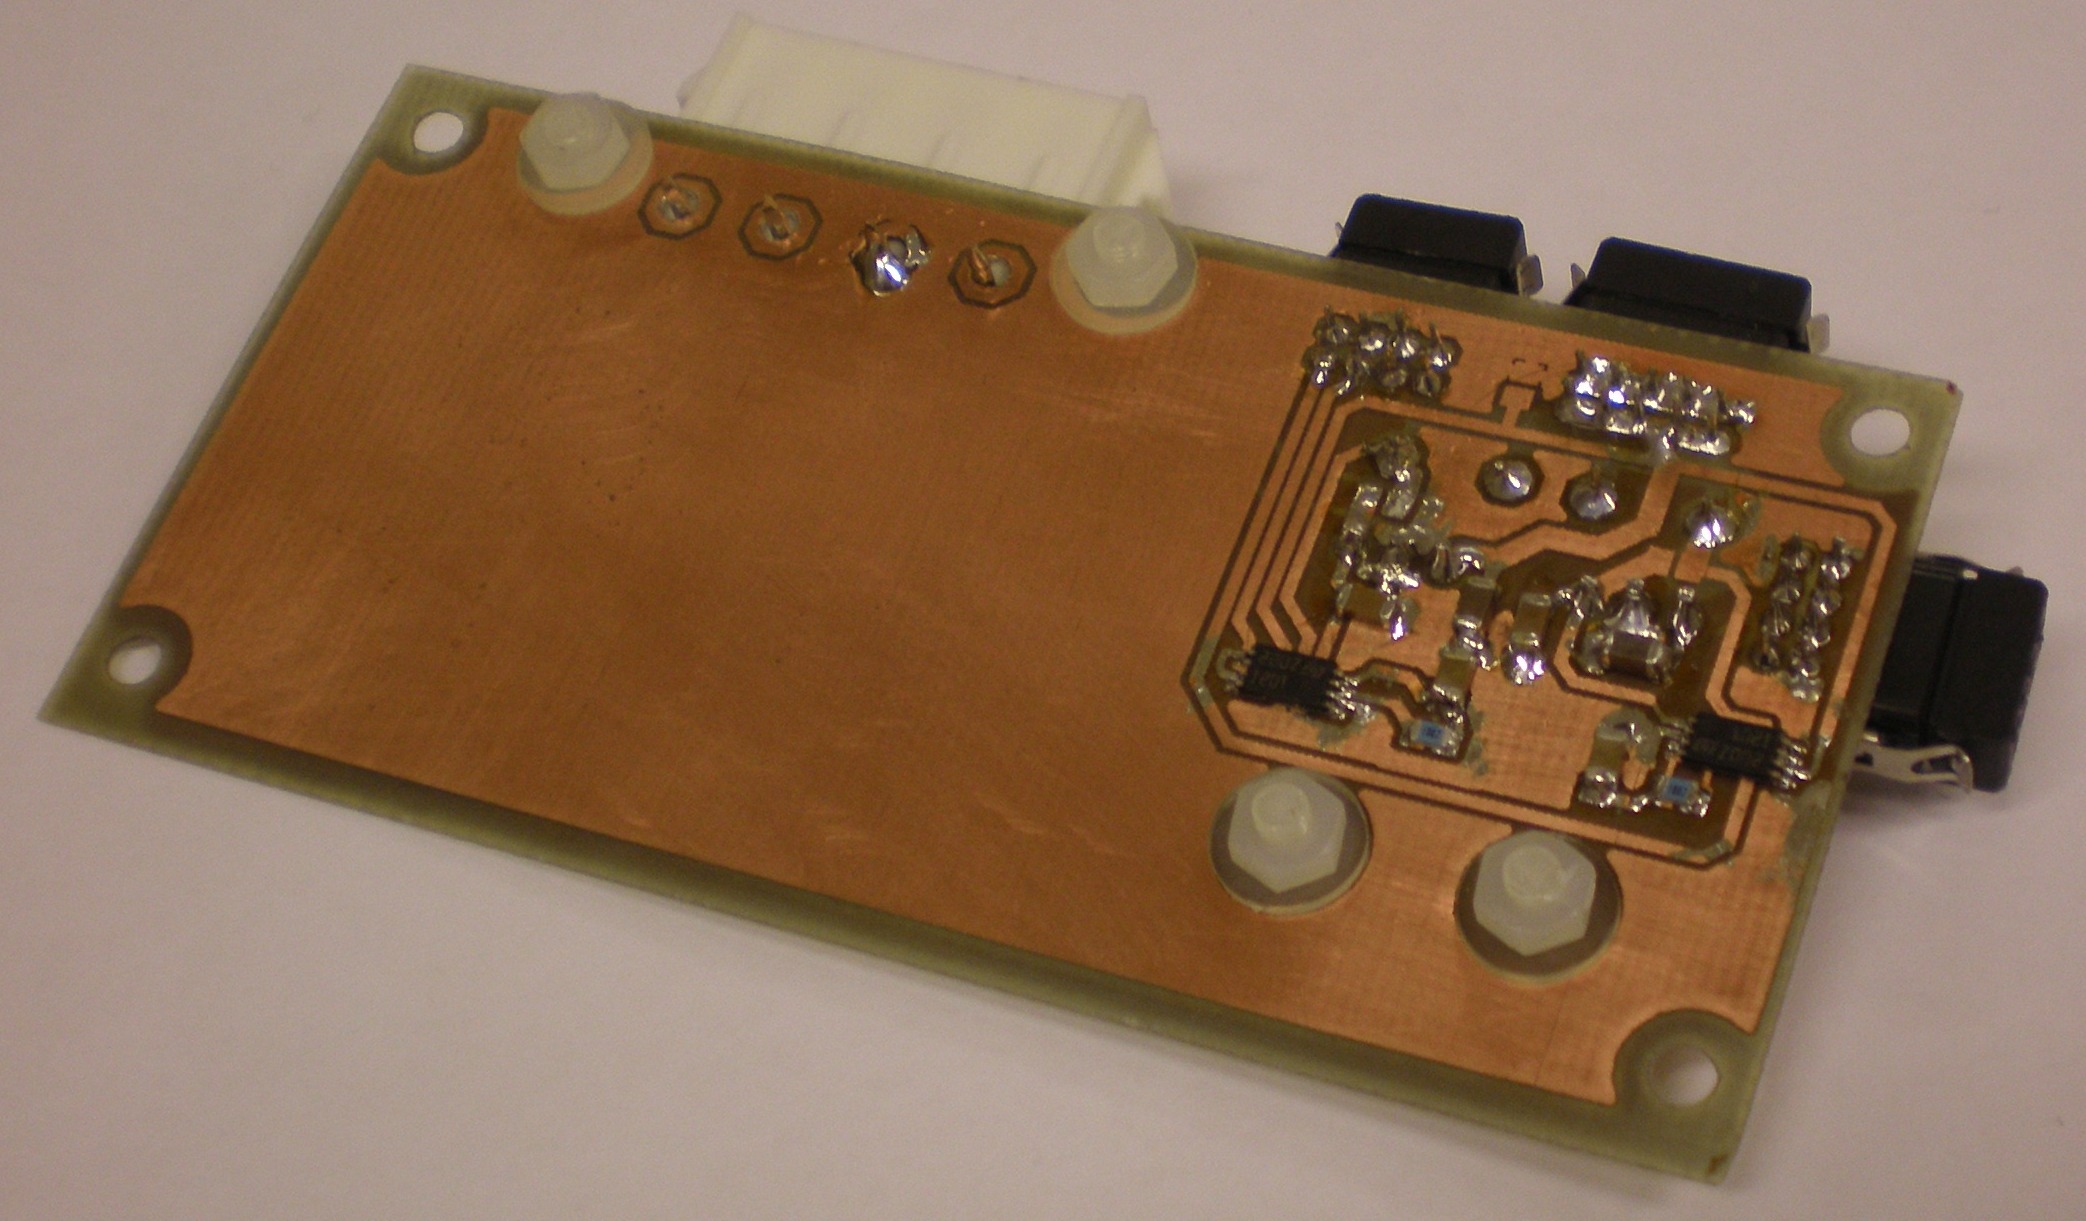
\includegraphics[width=0.7\textwidth]{figures/fig_SAR_bottom}
\end{minipage}
\caption{Battery Charge Regulator}
\label{fig:SAR_top_bottom}
\end{figure}

\begin{figure}[H]
\centering
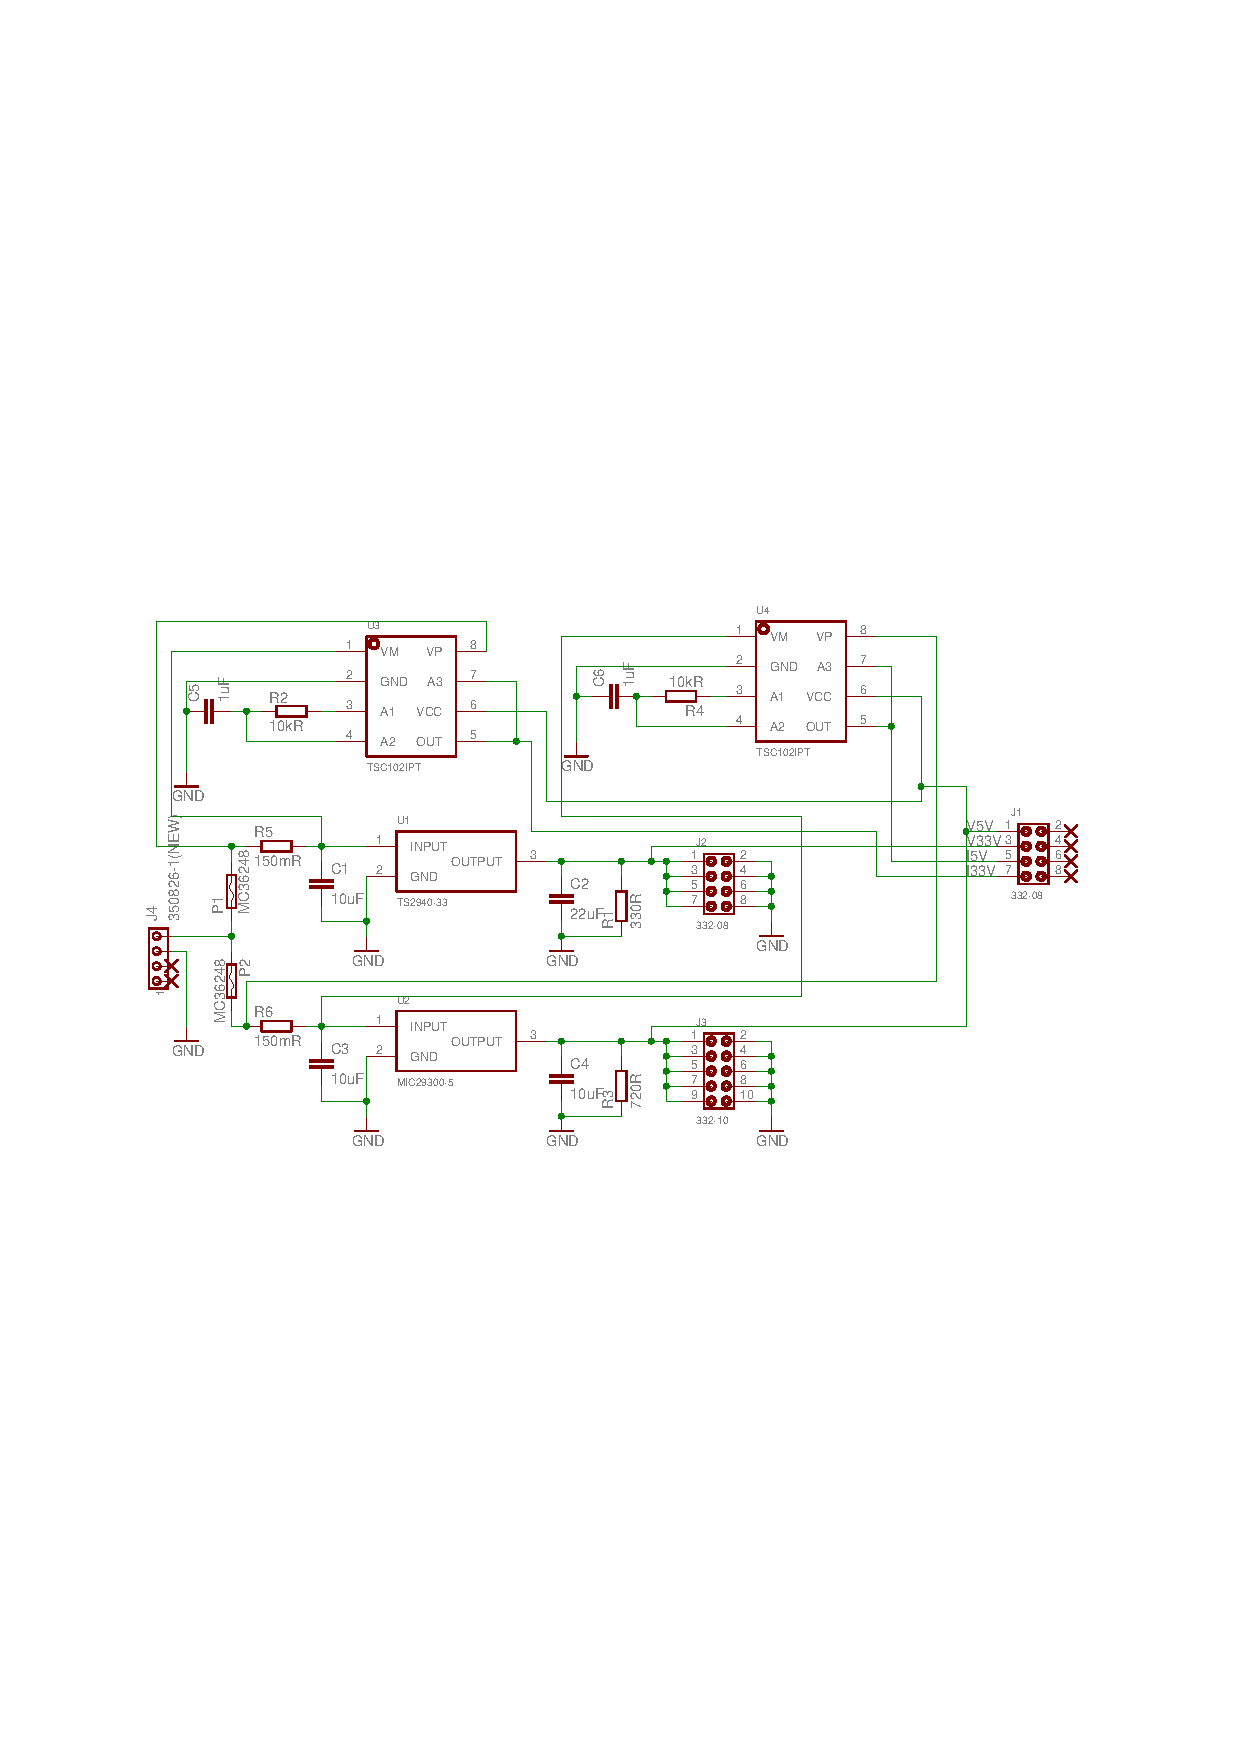
\includegraphics[width=\textwidth]{figures/fig_Schematic_SAR}
\caption{Schematic of the \acl{SAR}}
\label{fig:SAR_Schematic}
\end{figure}


\subsection{Temperature Sensor Board}


\begin{figure}[H]
\centering
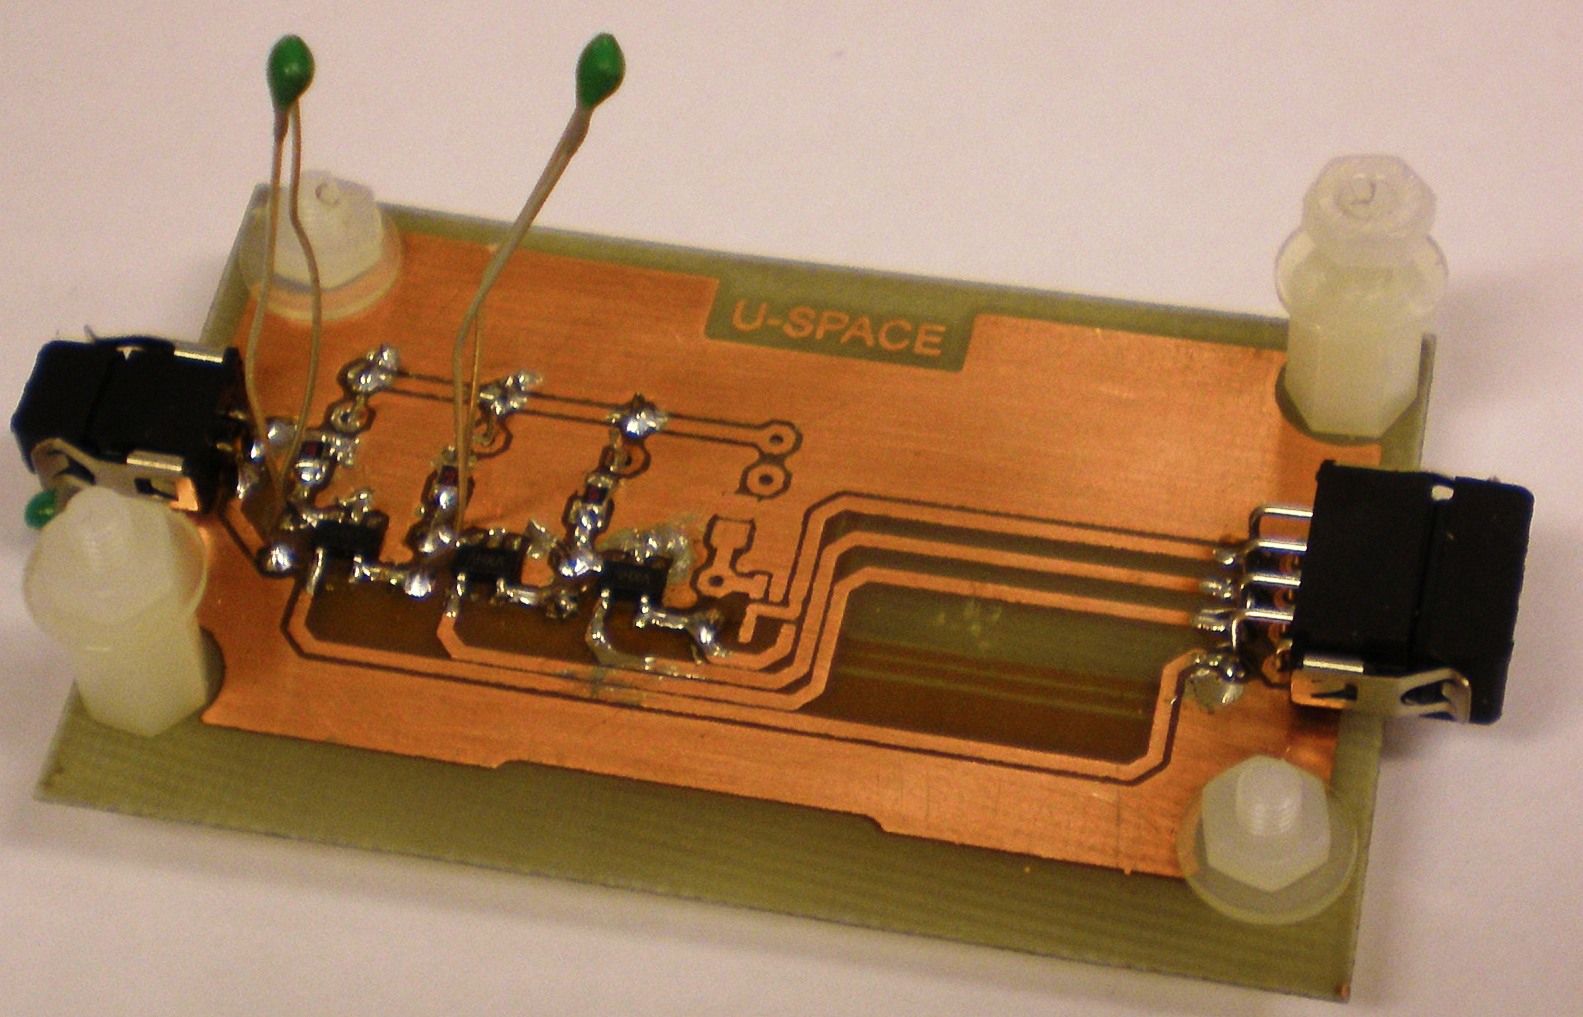
\includegraphics[width=0.7\textwidth]{figures/fig_Temp_top}
\caption{Temperature Sensor Board}
\label{fig:TS_top}
\end{figure}

\begin{figure}[H]
\centering
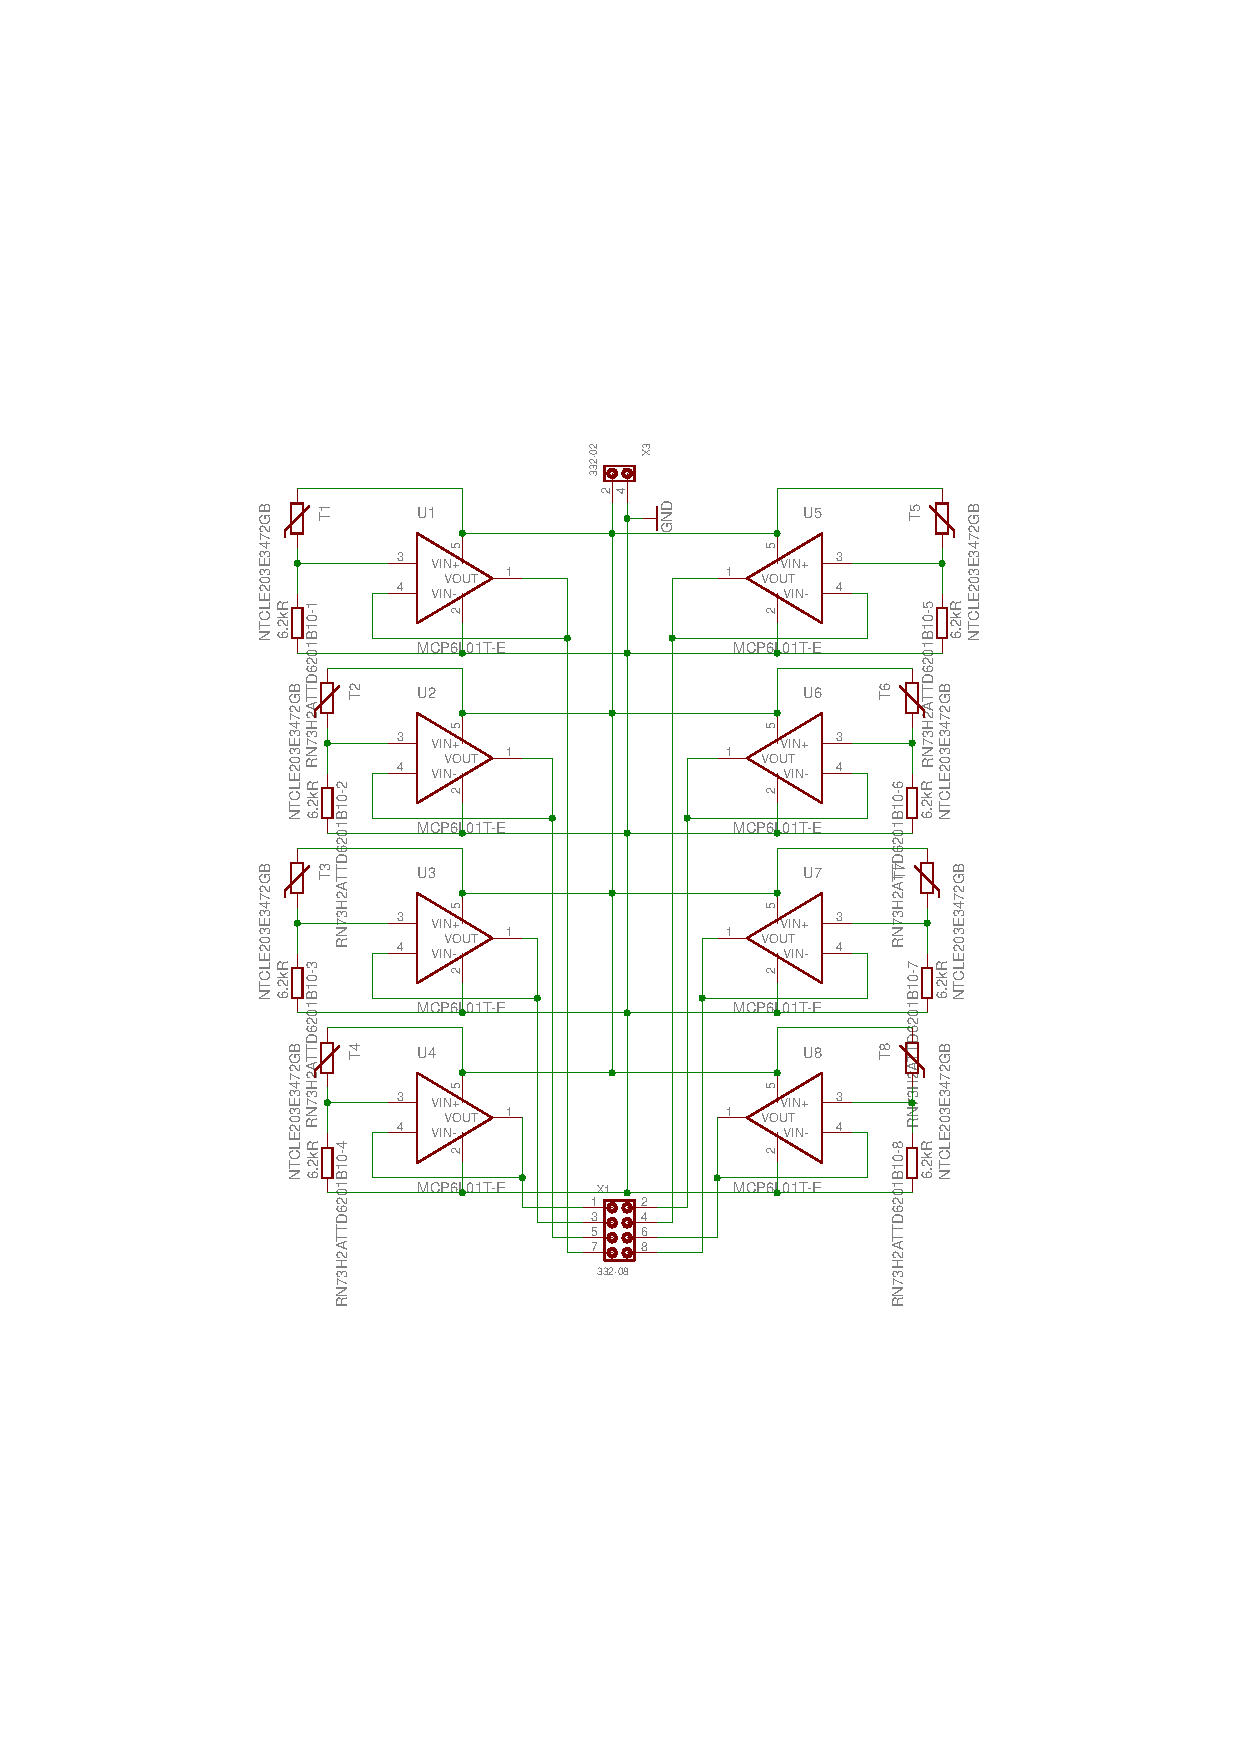
\includegraphics[width=\textwidth]{figures/fig_Schematic_TS}
\caption{Schematic of the Temperature Sensor Board}
\label{fig:Schematic_TS}
\end{figure}


\section{Mechanical Structure and Envelope}
%responsible: Pedro 

\section{Motor Control and Communication}
%responsible: Pedro and Morten

Temperature monitoring not implemented due to lack of thin wire (ordered thin wire proved to be non-practical to work with = too fragile).


\section{Imaging and Tracking Payload Unit}
%responsible: Jan

\section{Telecommunication}
%responsible: Omair